\documentclass[11pt,a4paper]{article}
\usepackage{fontspec}
% Pagella's book-style serif is paired with matching OpenType mathematics.
\setmainfont{TeX Gyre Pagella}[Ligatures=TeX]
\setsansfont{TeX Gyre Heros}[Scale=MatchLowercase]
\setmonofont{TeX Gyre Cursor}[Scale=MatchLowercase]
\usepackage{microtype,amsmath,mathtools,graphicx,booktabs,longtable,array}
\usepackage[warnings-off={mathtools-colon,mathtools-overbracket}]{unicode-math}
\setmathfont{TeX Gyre Pagella Math}
\usepackage{xcolor,titlesec,fvextra,needspace}
\DefineVerbatimEnvironment{CNSAlgorithm}{Verbatim}{fontsize=\footnotesize,breaklines=true,breakanywhere=true,frame=lines,framesep=3mm}
\definecolor{CNSInk}{HTML}{243446}
\definecolor{CNSBlue}{HTML}{0F4D92}
\definecolor{CNSMuted}{HTML}{526173}
\titleformat{\section}{\large\sffamily\bfseries\color{CNSInk}}{\thesection}{0.75em}{}
\titleformat{\subsection}{\normalsize\sffamily\bfseries\color{CNSInk}}{\thesubsection}{0.75em}{}
\titlespacing*{\section}{0pt}{2.0ex plus .7ex minus .2ex}{1.0ex plus .2ex}
\titlespacing*{\subsection}{0pt}{1.6ex plus .5ex minus .2ex}{0.7ex plus .2ex}
\linespread{1.04}
\clubpenalty=10000
\widowpenalty=10000
\displaywidowpenalty=10000
\usepackage[a4paper,margin=26mm,headheight=14pt,footskip=18pt]{geometry}
\usepackage{enumitem}
\setlist{nosep,leftmargin=*}
\usepackage{float,caption}
\captionsetup{font={small},labelfont={sf,bf},skip=8pt}
\usepackage[section]{placeins}
\usepackage[round]{natbib}
\setcitestyle{numbers,square,sort&compress}
\usepackage{fancyhdr}
\pagestyle{fancy}
\fancyhf{}
\fancyhead[L]{\footnotesize\sffamily\color{CNSMuted} TRACE · Research proposal · v0.1}
\fancyhead[R]{\footnotesize\sffamily\color{CNSMuted} GTCode.com}
\fancyfoot[C]{\small\sffamily\color{CNSMuted}\thepage}
\renewcommand{\headrulewidth}{0.3pt}
\fancypagestyle{opening}{\fancyhf{}\renewcommand{\headrulewidth}{0pt}\fancyfoot[C]{\small\sffamily\color{CNSMuted}\thepage}}
\usepackage[unicode,pdfencoding=auto,colorlinks=true,linkcolor=CNSBlue,citecolor=CNSBlue,urlcolor=CNSBlue]{hyperref}
\hypersetup{
 pdftitle={TRACE: Contrast-Guided Discovery from Conflicting Accounts},
 pdfauthor={GTCode.com},
 pdfsubject={Unvalidated research proposal, version 0.1; no TRACE experiments reported},
 pdfkeywords={TRACE, predictive synthesis, falsification, research proposal},
 pdfcreator={LuaLaTeX / GTCode.com}
}
\urlstyle{same}
\newcommand{\CNSIdentifier}[1]{{\small\ttfamily\def\_{\textunderscore\allowbreak}#1}}
\providecommand{\tightlist}{\setlength{\itemsep}{0pt}\setlength{\parskip}{0pt}}
\emergencystretch=1.2em
\setlength{\parskip}{0.42em}
\setlength{\parindent}{0pt}
% A flush-left title block and full-width abstract replace article's indented
% quotation-style abstract. All layout choices live in this editable source.
\renewenvironment{abstract}{%
  \par\vspace{1.1em}%
  {\sffamily\bfseries\color{CNSInk} Abstract\par}%
  \vspace{0.35em}\small\setlength{\parindent}{0pt}\noindent\ignorespaces
}{\par\vspace{0.9em}\normalsize}
\begin{document}
\thispagestyle{opening}
\begingroup
\raggedright
{\small\sffamily\bfseries\color{CNSBlue} RESEARCH PROPOSAL\enspace /\enspace VERSION 0.1\par}
\vspace{1em}
{\fontsize{27}{31}\selectfont\bfseries TRACE\par}
\vspace{0.55em}
{\Large Contrast-Guided Discovery\par}
\vspace{0.18em}
{\large from Conflicting Accounts\par}
\vspace{0.9em}
{\normalsize\sffamily GTCode.com\enspace ·\enspace 15 November 2026\par}
\vspace{0.55em}
{\small\sffamily\color{CNSMuted} Conceptual framework · Not empirically evaluated\par}
\endgroup
\vspace{0.8em}
{\color{CNSBlue}\hrule height 0.7pt}
\begin{abstract}
Conflicting reports can expose measurement differences, copied evidence
or omitted explanatory conditions. \textbf{TRACE (Testing Rival Accounts
through Contrast and Evidence)} investigates whether explicitly locating
these differences improves discovery beyond established contrastive and
abductive methods given the same source evidence and resources. The
procedure aligns claims, accounts for evidence lineage, generates rival
explanations and tests committed predictions. Its primary comparison
adds a generated conflict record to a common contrastive-discovery
scaffold, holding downstream selection and prediction scoring fixed.
Further comparisons distinguish lineage handling, extraction and
candidate ordering. Success requires a measurable explanatory
relationship absent from the source packet and accurate predictions on
sealed observations. The proposed first study uses 12--20 development
cases followed by a separate 30--60-case exploratory pilot. Reliability
measures constrain interpretation; adaptive investigation and larger
studies depend on the pilot's findings. TRACE integrates established
techniques and proposes a test of their incremental value. No
implementation or experiments are reported, and neither superiority nor
methodological novelty has been established.
\end{abstract}

\section{Introduction: when disagreement is
informative}\label{introduction-when-disagreement-is-informative}

Imagine one report stating that enabling a cache reduces request latency
and another reporting that it increases latency. Both statements can be
compatible with reality if request reuse, update frequency, resource
pressure, or freshness constraints differ. They can also be incompatible
because a measurement is faulty, a source copied erroneous numbers, or
one account simply makes a false generalization. The correct response is
not necessarily reconciliation. A system ought to distinguish different
questions, reject unsupported accounts when warranted, and preserve
genuinely unresolved alternatives.

This example exposes a gap between \emph{answer selection} and
\emph{explanatory discovery}. Selecting the more credible report can be
useful. So can identifying the source of a contradiction or expressing
uncertainty. An established goal of abductive research is to infer a
\textbf{measurable condition} not stated in either report, state what
new observations that condition predicts, and seek an observation
capable of refuting it. If the condition merely redescribes the evidence
already seen, no discovery has occurred. If the model uses hidden
evaluation labels to invent it, the result is invalid. If a simple
fitted regression does as well, the more elaborate synthesis process has
not justified its cost.

The \emph{Against All Likelihood} essay by Lopez-Paz argues that
language likelihood is neither necessary nor sufficient for objective
truth and explores invariance across relevant transformations as a guide
to more robust knowledge \citep{R01}. That argument motivates testing an
account across contexts, but does not by itself resolve the crucial
question of \textbf{which transformations should preserve which aspect
of an answer}. A stable false statement survives every harmless
paraphrase. A correct account may need to change after a new measurement
or a regime shift. For TRACE, this suggests that truth-seeking requires
both robustness to irrelevant differences and correct responsiveness to
relevant differences---not a blanket rule that all answers should agree.

Earlier CNS work proposes synthesizing Structured Narrative Objects,
rather than merely voting on isolated claims. It includes critics,
evidence grounding, access states, predicate invention subject to stated
limits, and the possibility of unresolved contradiction
\citep{G02, G03, G11}. TRACE retains those useful aims while shifting
the scientific burden to new predictions and comparisons with ordinary
alternatives. An independent evaluator must measure whether the
procedure improves predictive outcomes.

\textbf{Why begin with narrative disagreement?} Sparse reports can
contain clues about omitted conditions that are absent from a ready-made
table. TRACE proposes that comparing opposing accounts can focus a
finite search over those clues. This is a mechanism hypothesis,
especially relevant when measurements are scarce and candidate
moderators are numerous, not a theorem that prose beats tabular
learning. Shared false assumptions, copied reports or abundant
well-measured structured data may remove the benefit. A common-extractor
learner and generic hypothesis-refinement comparator must receive the
same records and budget; matched contradiction-uninformative packets
test whether disagreement adds value beyond hypothesis generation
itself.

\textbf{Method in brief.} TRACE records where accounts differ in target,
evidence lineage, assumptions and explanatory relationships. Its
generator uses those contrasts to propose explanations with measurable
variables and distinguishing predictions. Acquisition can supply
initially missing context, while warrant remains separate from
hypothesis generation. Sections 4.1--4.6 specify the record types,
generator interface, numerical compiler, action policy and stopping
states. The primary research question concerns the incremental
predictive value of localized source disagreement beyond existing
discovery methods; generation and ordering experiments distinguish
possible mechanisms behind any improvement.

\textbf{Scope.} The proposed procedure addresses empirical claims with
explicit target variables, accessible records, or feasible observations.
It does not claim a universal criterion of truth, solve disputes of
values, or recover causal structure without identification assumptions.
We propose a concrete representation, a discovery loop with fixed search
and action budgets, and an evaluation whose failure would count against
central TRACE claims. No experimental findings are offered here.

\section{Related work and contribution
boundary}\label{related-work-and-contribution-boundary}

\subsection{Closest source-conflict and discovery
precedents}\label{closest-source-conflict-and-discovery-precedents}

Contrastive Discovery represents a scientific question through competing
explanations and uses evidence-induced belief redistribution to evaluate
and guide discovery \citep{R41}. Its data-and-metadata experiments
directly precede TRACE's rival-comparison loop. TRACE cannot claim
priority for contrastive experimentation; the proposed distinction is
the incremental value of source-conflict localization, tested without
withholding source facts from that comparator.

POPPER implements agentic falsification with sequential statistical
safeguards \citep{R42}. Its guarantees require valid implications and
conditionally valid tests; TRACE's deterministic set-separation
heuristic does not inherit those guarantees. A later investigation study
must compare against a faithful POPPER adaptation wherever valid
statistical tests are available, and report task incompatibilities
instead of replacing it with a weak prompt.

Claim Cards records explicit interpretations before evidence gathering
\citep{R43}. ConfRAG evaluates reasoning over conflicting web references
\citep{R44}. Perceive-Then-Adjudicate addresses conflicts between model
knowledge and retrieved evidence \citep{R46}. These precedents constrain
claims for alignment, conflict organization and agent arbitration; their
outcomes are not equivalent to new held-out predictive conditions.

Contradiction-driven explanation itself is established: Behfar and
Okhuysen discuss abductive inquiry into discordant findings \citep{R47}.
PARADOX analyzes pharmacological contradictions and contextual
differences \citep{R48}. The publisher links an official repository
containing sentence-pair classification, iterative refinement, GPT
contradiction checking and graph construction. In the inspected
evaluation notebook, the reference labels are GPT labels, not
independent outcome measurements. No committed held-out
condition-prediction workflow was identified in the inspected notebooks.
The full article remains subscription-only, so this implementation
inspection does not settle full-method differentiation. Contextual
reconciliation is already prior art; TRACE must establish added
predictive value. Earlier clinical work also uses ChatGPT to
differentiate conflicting scientific evidence \citep{R49}. Failing to
Falsify supplies a required simple counterexample-prompting control
\citep{R45}.

\textbf{Contribution boundary.} The remaining question is whether a
particular representation of documented disagreement improves candidate
generation and independently predictive scope discovery under matched
information and cost. Neither source independence nor useful
localization is assumed from a citation count. The
\href{https://gtcode.com/papers/trace/prior-art-audit.md}{prior-art
audit} records inspection depth, assumptions and access gaps; the
\href{https://gtcode.com/papers/trace/contribution-matrix.md}{contribution
matrix} assigns each proposed contribution a precedent and a comparison
that could eliminate it. These are targeted searches, not an exhaustive
novelty certificate.

\subsection{Invariance and its
limitations}\label{invariance-and-its-limitations}

Invariant causal prediction studies stable relationships under
environmental changes subject to explicit assumptions about the causal
system \citep{R03}. Invariant Risk Minimization (IRM) proposes a
representation in which the same predictor is optimal across training
environments \citep{R02}. These precedents motivate the question,
``Which relationship remains useful under which changes?'' They do
\textbf{not} show that passing prompt-paraphrase tests establishes world
truth, or that the prompt context generated by a language model is
equivalent to an observed intervention. Negative analyses of IRM and
comparisons with tuned empirical-risk baselines are central warnings
against treating invariance as a solved optimization problem
\citep{R04, R05, R06}. Work on discovering environments adds possible
future tools but not a reliable admissibility oracle \citep{R07}.

Lopez-Paz motivates the joint investigation of explanations and
admissible transformations, including the use of new predictions and
attempted falsification \citep{R01}. TRACE adopts that motivation; it
does not claim these principles as original contributions. His
inference-time sketch generates answers under varied contexts and
extracts an invariant core. TRACE proposes a different operational
procedure: retain competing scoped explanations, commit their
distinguishing predictions before acquiring outcomes, and select
evidence-gathering actions using a specified rival-separation rule.
Explicit provenance, transformation contracts, and failure states make
that procedure inspectable. Whether this combination improves predictive
synthesis or investigation over simpler alternatives remains an
empirical question.

Behavioral testing supplies a practical precedent for structured
perturbations, and counterfactually augmented examples distinguish
robust behavior from sensitivity to superficial cues \citep{R08, R09}.
However, a transformation that removes the only relevant source is not a
mere nuisance. Neither is changing a measured causal input. A benchmark
must state the expected response for each transformation instead of
rewarding identical strings under every condition.

\subsection{Evidence, source dependence, and warranted
assertion}\label{evidence-source-dependence-and-warranted-assertion}

Retrieval-augmented generation and chain-of-verification can help
connect an answer to accessible evidence \citep{R11, R16}. Source
dependence is a separate issue: many reports may reproduce the same
originating record and therefore should not be treated as independent
confirmations \citep{R10}. This is particularly important when a
seemingly broad consensus is produced by copying. TRACE distinguishes
(i) whether two claims address the same estimand, (ii) whether they rely
on the same record, and (iii) whether nominally distinct sources share a
lineage. These are not interchangeable quantities.

A cited source can establish that a statement \textbf{was reported}, not
that the statement is automatically correct. Likewise, a valid deduction
from premises remains conditional on the premises. SNOs therefore
preserve exact source spans, time, access and dependency, while a
separate warrant field records whether the claim is source-reported,
derived given premises, empirically supported within scope, refuted
within scope, or unresolved. Existing CNS 8.0 material recognizes the
distinction between an internally stable orthesis and metaphysical
truth; our proposal makes predictive and observation-based tests
additional explicit gates, not a retrospective claim that the prior work
ignored uncertainty \citep{G02, G03, G08}.

\subsection{Aggregation, debate, abduction, and
argumentation}\label{aggregation-debate-abduction-and-argumentation}

Self-consistency aggregates multiple reasoning samples; debate
structures disagreement between models; verification asks targeted
subquestions \citep{R12, R13, R16}. Results of multi-agent comparisons
suggest that debate must be compared against simpler voting or
aggregation rather than credited with improvement by default
\citep{R14}. Model-generated reasons can also be unfaithful to the
causes of a model's answer \citep{R18}, so TRACE audits short,
externally checkable justifications rather than treating hidden
reasoning traces as evidence.

The distinction between supporting and attacking arguments has a long
formal tradition in abstract argumentation \citep{R32}. Abductive
inference generates candidate explanations from observations;
computational forms include cost-based first-order abduction
\citep{R33}. Inductive logic programming (ILP) supplies a precedent for
rule and predicate learning in a specified language \citep{R21}. These
traditions already cover substantial ground claimed informally by many
``discovery'' systems. TRACE does not claim to invent abduction,
argument attacks, or predicate invention. The proposed artifact is a
procedure and comparative design for testing
\textbf{conflict-conditioned predictive discovery}. Combining familiar
components does not establish methodological novelty. The empirical
question is whether explicit source-conflict localization adds
predictive value beyond those methods.

Iterative hypothesis generation is already a close precedent. HypoGeniC
updates a bank of natural-language hypotheses using prediction errors on
labeled examples \citep{R37}. Qiu and colleagues propose, select and
refine rules with symbolic interpretation, distinguishing rule induction
from reliable application \citep{R38}. These methods motivate a required
refinement comparator, rather than treating discovery as a comparison
only with answer aggregation. Causal Modelling Agents combine LLM
metadata reasoning with data-driven structural causal models
\citep{R39}; that is relevant hybrid causal-modeling precedent, not
evidence for the proposed TRACE procedure or a universal intervention
capability.

\subsection{Choosing observations and existing discovery
agents}\label{choosing-observations-and-existing-discovery-agents}

AutoDiscovery already generates contexts, derived variables and
relationships, including hypotheses across datasets; its released
implementation also defines structured hypothesis dimensions
\citep{R50}. These capabilities are inherited, not distinctive to TRACE.
Its search uses model belief change, which is not an external
correctness label. A credible comparator must retain its ability to
propose conditional explanations. Piriyakulkij and colleagues combine
LLM-proposed natural-language rules, probabilistic belief updates and
experiment design \citep{R40}. This is a close precedent for the
hypothesis--experiment loop. TRACE therefore tests the added value of
explicit comparison between source accounts, including their measurement
and lineage differences, rather than claiming to originate automated
experimentation.

Bayesian experimental design gives a principled account of selecting
actions to reduce uncertainty when the relevant hypotheses, likelihoods
and priors can be specified \citep{R20}. Active learning for causal
structure makes the experimental-choice problem concrete \citep{R31}.
TRACE uses a set-separation heuristic when probability models are
unspecified and compares it with relevance-based and random acquisition.
Predicting intervention outcomes does not by itself identify a causal
graph.

Modern work already explores agentic scientific workflows: \emph{The AI
Scientist} automates parts of idea generation, experimental code and
reporting \citep{R34}; \emph{Co-Scientist} develops scientific
hypotheses through agent coordination and evaluation \citep{R35}; and
\emph{Robin} connects literature agents, analysis and experimental
biology \citep{R36}. These workflows provide established alternatives
for hypothesis generation and experiment planning. TRACE focuses on the
additional value of explicitly locating disagreement in their source
evidence. DiscoveryBench provides a separate transfer diagnostic, while
FEVER, SciFact and AVeriTeC test forms of source-grounded verification
rather than universal truth \citep{R25, R26, R27, R28}.

\section{Epistemic commitments and
nonclaims}\label{epistemic-commitments-and-nonclaims}

Four distinctions govern the proposal.

\textbf{Truth is not identical to current warrant.} Whether a scoped
proposition is true in the world is separate from whether the available
record supports saying so. The system can update warrant after evidence
arrives without changing the historical fact being described. A true
claim with inaccessible support remains unwarranted; a previously strong
citation can later be retracted.

\textbf{Coherence is not correctness.} Propositions can agree because
they share a mistaken assumption, training artifact or copied source. A
stable internal model can be a sensible computational stopping
condition, not proof of objective truth. This applies to deductive
closure, round-trip translation, majority vote, and invariance over
model-generated perspectives.

\textbf{Stable mechanism is not constant output.} A representation-only
nuisance change should preserve the relevant meaning, up to an explicit
transformation of units or format. If the population, intervention or
measurement changes, a credible explanation may predict a
\emph{different} outcome. If a unique support record disappears, the
empirical event need not change but the warrant may weaken. We therefore
use transformation-specific output relations.

\textbf{Uncertainty is not lack of access.} Observation noise,
unavailable records, open-world ambiguity, and observationally
equivalent mechanisms imply different limitations. Two worlds that
supply exactly the same permitted observations but require different
conclusions cannot be separated merely by more model deliberation. The
legitimate output may be a set of live alternatives and an
identification boundary.

TRACE treats a proposed new scope condition as a hypothesis until its
operands are observable and it has predictive consequences not exhausted
by the source examples. A cause is not identified merely because a story
explains a correlation. A probabilistic forecast must refer to a
specified event; token likelihood is not used as its substitute. These
commitments are falsifiable at the level of system behavior and
externally measured outcomes; they are not axioms purportedly
guaranteeing truth.

\section{Method: alignment, explanation generation and
investigation}\label{method-alignment-explanation-generation-and-investigation}

\subsection{Four-stage procedure and common
records}\label{four-stage-procedure-and-common-records}

TRACE asks whether comparing the explanatory structure of conflicting
accounts helps generate independently predictive explanations. Its four
stages are \textbf{alignment}, \textbf{lineage accounting},
\textbf{rival generation}, and \textbf{investigation with warrant
assignment}. The numerical compiler in Section 4.4 is one component of
rival generation. Cases can stop at any stage with a recorded reason;
successful normalization alone does not count as explanatory discovery.

A question is \(q=(Y,\mathcal P,t,\mathcal I,u,\tau)\): outcome
definition and aggregation, population, time/window, intervention or
observation context, units and tolerance. An evidence atom records its
source, exact span or measurement, timestamp, access state, measurement
lineage and collection context. A report contains atomic claims,
assumptions and asserted explanatory relationships, each linked to
evidence atoms. The record distinguishes \CNSIdentifier{source\_stated} content
from \CNSIdentifier{extractor\_inferred} interpretation. Neither attribution
nor extraction establishes truth.

\textbf{Stage A: alignment.} Compare the questions and create a conflict
record \(\Delta(A,B)\). Its \CNSIdentifier{estimand\_status} is \CNSIdentifier{same},
\CNSIdentifier{unit\_convertible}, \CNSIdentifier{different} or \CNSIdentifier{unknown}. A
unit mapping records its formula and preconditions; apply it only when
the outcome definition, aggregation and relevant scope match. Median and
p99 are different targets, not convertible units. Preserve them as
separate questions unless the required underlying distribution is
available. Different context populations may motivate a transport/scope
hypothesis; do not silently treat their observed effects as
contradictory measurements of one fixed population. Record separately
whether the sources assert incompatible generalizations, whether their
observed intervals differ, and what context differences might explain
the contrast.

\textbf{Stage B: lineage accounting.} Record \CNSIdentifier{shared\_origin},
\CNSIdentifier{distinct\_origins}, \CNSIdentifier{mixed} or \CNSIdentifier{unknown}, with
evidence for each lineage link. Collapse only duplicate measurements,
retaining source attribution and any additional observations. Distinct
origins do not guarantee statistical independence. Copied support
contributes once; copying does not refute the claim, validate its rival,
or identify the true mechanism. Unknown dependence remains explicit and
receives prespecified sensitivity analysis. A defective measurement can
be excluded only for a recorded defect criterion; the exclusion does not
establish the competing account.

\textbf{Stage C: rival generation.} Use the report claims, assumptions,
relationships and conflict record to propose conditional explanations or
rival mechanisms (Section 4.3). Variables can enter through three
provenance states: \CNSIdentifier{observed\_shared} (values recorded in both
accounts), \CNSIdentifier{observed\_asymmetric} (recorded in one but missing in
another), or \CNSIdentifier{inferred\_unmeasured} (proposed, with no measured
values). These states apply relative to the cited report pair;
cell-level missingness remains recorded. A variable's
\CNSIdentifier{conflict\_ids} lists applicable conflict records and may be
empty during extraction. If its provenance state differs across pairs,
use pair-specific variable records linked to the same operational
definition. Observed in prose need not mean numerically fit-ready. No
missing value may be inferred merely because an explanation needs it.

\textbf{Stage D: investigation and adjudication.} Commit testable
predictions, acquire permitted observations and update claim-specific
warrant. A candidate requiring new measurements remains pending until it
can predict or be fitted. A case with no available identifying
observation remains unresolved. Runtime cannot certify global
non-identifiability; that classification belongs to the sealed
evaluator. Runtime records which alternatives remain and why its
permitted actions cannot separate them.

\textbf{Common export.} Every run uses the same linked tables, including
runs that never generate a fitted rule. IDs join records within a case;
null denotes unknown, never false or zero.

\begin{longtable}[]{@{}
  >{\raggedright\arraybackslash}p{(\linewidth - 2\tabcolsep) * \real{0.5000}}
  >{\raggedright\arraybackslash}p{(\linewidth - 2\tabcolsep) * \real{0.5000}}@{}}
\toprule\noalign{}
\begin{minipage}[b]{\linewidth}\raggedright
Table
\end{minipage} & \begin{minipage}[b]{\linewidth}\raggedright
Required scientific content
\end{minipage} \\
\midrule\noalign{}
\endhead
\bottomrule\noalign{}
\endlastfoot
\CNSIdentifier{questions}, \CNSIdentifier{evidence}, \CNSIdentifier{reports} & Target/scope;
source spans and measurements; claims, assumptions and explanatory
relations with attribution type \\
\CNSIdentifier{conflicts} & Report and question IDs; estimand and lineage
statuses; incompatible claims; context differences; transformations and
unresolved fields \\
\CNSIdentifier{variables}, \CNSIdentifier{observations} & Definition, units/type,
provenance state and measurement procedure; observed values, time and
lineage, including missing cells \\
\CNSIdentifier{candidates} & Conflict IDs; retained/rejected claim IDs; added
relationship; assumptions; variable IDs; executable prediction or
pending dependencies; generation rank and status \\
\CNSIdentifier{predictions}, \CNSIdentifier{actions} & Candidate, target and action
IDs; prediction region, tolerance, commitment time; requested
measurement, response and cost \\
\CNSIdentifier{decisions} & Stage, affected claim IDs, reason, evidence IDs,
warrant and unresolved alternatives \\
\CNSIdentifier{scores} & Evaluator-only outcomes, errors, endpoint verdicts and
mechanism-family strata, appended after commitment \\
\end{longtable}

The downloadable
\href{https://gtcode.com/papers/trace/trace-records.schema.json}{record
schema} defines these fields and types. Referential integrity,
source-span fidelity, units and temporal availability are semantic
requirements beyond JSON shape validation. Candidate and decision traces
describe program operations, not private model reasoning. Aggregate by
independent root, not by the number of candidates or observations. This
allows the same analysis to distinguish alignment corrections,
dependence adjustments, new conditions, refuted candidates and
unresolved cases across F1--F8 without passing family labels to runtime.

\textbf{Role of the architecture.} Alignment and provenance accounting
implement inherited safeguards. Stage C is the principal experimental
target: does an explicit conflict record improve the proposed conditions
and their predictions? Stage D implements investigation using
established experimental-design ideas. Neither multiple agents nor the
numerical compiler is required to be an innovation. The primary
mechanism comparison in Section 8 holds downstream compilation and
evaluation fixed; a separate end-to-end comparison measures the cost and
errors of producing the conflict record itself.

\subsection{Transformation contracts}\label{transformation-contracts}

Three records must remain separate. A
\textbf{representation/evidence-integrity contract}
\(c_T=(T,\operatorname{pre}_T,r_T,v_T,z_T)\) declares an operation,
preconditions, a property that should be preserved or converted, a
validator and a state
\(z_T\in\{\text{validated},\text{rejected},\text{unknown}\}\). Unit
conversion can require numerical equivariance; a demonstrably redundant
copy must not count as another independent observation. The
preconditions matter: order can encode chronology, a paraphrase can
change scope, and a copied document can contain new evidence. Semantic
validity is not universally decidable by deterministic code. Removing
evidence can change warrant, but does not impose a universal direction
of confidence change.

A \textbf{rival-indexed response commitment} \(r_{T,h}\) states how
hypothesis \(h\) predicts an outcome will respond to a world, regime or
evidence change. Different rivals may make incompatible commitments. The
runtime need not know which mechanism is true before recording that
disagreement. Knowing that an operation preserves units does not
establish that a disputed world change preserves the outcome.

An \textbf{evaluator-only relation} specifies the benchmark's expected
behavior from its sealed state. It scores the method after outputs are
locked and is never passed to runtime as a validated contract.
Gold-admissibility access is a diagnostic ceiling, excluded from
superiority claims.

For a representation/evidence-integrity contract, the check remains
three-valued:

\[
C_T(x)=\begin{cases}
\mathrm{pass},&z_T=\mathrm{validated}\text{ and }r_T\text{ is verified},\\
\mathrm{fail},&z_T=\mathrm{validated}\text{ and }r_T\text{ is violated},\\
\mathrm{unknown},&\text{the contract or necessary evidence is unresolved}.
\end{cases}
\]

For a rival-indexed commitment, the system records predictions and later
adequacy checks, not an oracle verdict about admissibility. Validators,
tolerances and expected evaluation relations must be frozen before
confirmation. A failed or unknown contract cannot be discarded merely
because its result is inconvenient.

\subsection{Rival generation and prediction
commitments}\label{rival-generation-and-prediction-commitments}

\textbf{Generator interface.} A run begins with one extraction call over
the permitted source packet. The extractor produces source-linked report
and observation records. Its instruction is: ``Preserve each account's
question, claims, assumptions and asserted relationships with exact
evidence IDs. Separate explicit statements from your interpretations.
Record missing or ambiguous values as null. Do not reconcile accounts or
supply absent measurements.'' Deterministic code performs verified unit
conversions, duplicate-measurement accounting and record joins;
uncertain semantic alignments stay unknown.

One generation call then receives the complete permitted packet, its
extracted records, the conflict records, the action menu and the
remaining budget. The instruction is: ``For each unresolved comparable
conflict, propose explanations that account for its observations. For
each candidate, identify the claims retained or rejected, the added
condition or relationship, its assumptions, and a prediction that
differs from a rival. Cite the conflict and evidence IDs motivating it.
Mark every added variable as observed\_shared, observed\_asymmetric or
inferred\_unmeasured. For missing measurements specify a procedure and
permitted action, or mark unavailable. Include an account-rejection
explanation only when evidence supports a defect; allow all accounts to
be inadequate. Output candidate records, not a consensus essay.''

The TRACE implementation permits up to eight proposals per generation
call, one schema-repair call containing only structural errors, and two
generation rounds in an adaptive run. A separate localization call turns
the extracted records into conflict records, cites supporting spans,
preserves unknowns and proposes no explanatory condition. Its tokens and
errors count toward the run. These call allocations describe TRACE and
the matched scaffold comparison; faithful method-level competitors can
allocate their calls differently within the same total resource ceiling.
A static run has one round and no acquisition. The second adaptive round
receives acquired observations and the preceding candidate records, with
old predictions immutable. These are proposed engineering limits, to be
fixed with the model version, inference settings and packet construction
before confirmation. Invalid or excess proposals remain logged and
consume generation budget; repairs cannot receive scoring outcomes.

\textbf{Variable acquisition.} An asymmetric variable cites the source
passage establishing its presence and the rows where its value is
missing. An unmeasured variable includes an operational definition,
units or categories, when it would be observed, motivating evidence or
an explicitly labeled mechanistic conjecture, and a permitted
measurement action if one exists. Neither variable state is a supported
explanation. After acquisition, update cell values and availability
while preserving the original provenance state. Missing context can
become a measured predictor within the run. If no permitted action can
supply it, record \CNSIdentifier{measurement\_unavailable} and retain
uncertainty rather than filling the column by inference.

\textbf{Candidate representation.} A candidate must explain which
original observations it accommodates, which claims it changes and why
its added relation would account for the difference. Prediction forms
are: a numerical expression over defined variables; a conditional rule;
or a categorical/interval commitment for a specified action. Executable
expressions use constants, variable IDs, arithmetic, comparisons and
conditional selection; division by zero or unavailable operands yields
an unknown prediction. No generated code executes outside this
expression interpreter. Parameters must be declared as fitted from
identified observations, source-specified, or conjectured. Conjectured
parameters can make testable predictions but acquire no empirical
warrant from being written down. Narrative-only candidates remain
\CNSIdentifier{pending\_prediction} and cannot earn H2 credit. Causal
candidates additionally declare intervention assumptions; predictive
success alone cannot establish a causal graph.

Candidate validity requires resolvable IDs, supported source
attributions, consistent units, an identified target and no use of
future outcomes. Semantic fidelity is assessed with a frozen rubric and
blinded independent adjudication for the study; these judgments score
the run and do not feed back into runtime. An explanation is allowed to
retain one account, reject both, introduce a scope condition or preserve
competing mechanisms. The parser enforces format and dependencies, not
truth.

\textbf{Prioritization.} At most four candidates are active for
investigation. Order valid proposals first by whether they address an
explicitly localized incompatibility, then by the number of distinct
observed report contexts they account for without an unsupported value
assignment, then by fewer newly assumed variables; break ties by
canonical candidate ID. These are auditable proposal features, not
calibrated truth probabilities. Include measurable pending candidates as
well as currently executable ones. Log all proposals and rankings so
candidate generation can be separated from selection effects. In the
complete TRACE procedure, select a final prediction candidate using the
same ordering among candidates that remain adequate; report unresolved
where none qualifies. The controlled C--B generation experiment replaces
this conflict-sensitive selector with the common selector specified in
Section 8.2. The numerical compiler may rank alternative parameterized
rules within a candidate using Section 4.4; its training score cannot
compare arbitrary prose mechanisms or confer warrant.

Before any scored observation is revealed, write a prediction commitment
\(k=(h,q,\hat y,\tau,a,t_0)\) with the candidate, question, prediction,
tolerance, action/context and timestamp. Preserve the record immutably.
Operational novelty requires a new relationship or scope condition and a
distinguishing consequence absent from the initial accounts; merely
translating units, extracting an existing qualification or changing a
source weight does not satisfy H2. An explanation must also account for
the motivating observations under its stated assumptions. Its held-out
predictions, rather than its rhetorical plausibility, determine
predictive success.

For task-appropriate loss \(\ell\), predictive error remains \[
R_e(M)=\mathbb E_{(x,y)\sim P_e}[\ell(M(x),y)].
\] Report risk alongside coverage and false promotions. A binary
world-event forecast can use Brier loss \((p-y)^2\) \citep{R22}; a
document-entailment confidence is a different quantity. The evaluator's
task definitions and tolerances are fixed before confirmation.

\subsection{Numerical rule compiler and search-order
experiment}\label{numerical-rule-compiler-and-search-order-experiment}

The numerical compiler implements one candidate form within Stage C. It
accepts numerical outcomes and predictor measurements available in every
fitting row, including variables measured through an earlier permitted
action. Other candidate forms use the prediction interface in Section
4.3. The compiler's restricted language does not define the full TRACE
architecture or cover every benchmark mechanism.

A compiled rule predicts one constant, or two constants separated by one
predicate or a conjunction of two predicates on distinct variables.
Numeric predicates use midpoints between consecutive observed values;
categorical predicates test equality to observed categories. Each
conditional branch requires at least two distinct measurement-lineage
units. Copy duplicates count once; repeated readings within a
lineage/context first form a mean. Missing cells produce
\CNSIdentifier{requires\_measurement}, not silent complete-case selection.
Record identifiers, source identities and target-derived variables
cannot be predictors. Numeric extrapolation, unseen categories and
missing prediction inputs return unknown under this compiler.

For the complete lineage-aware procedure (D), fit branch constants by
weighted least squares and rank fitted alternatives by \[
J(g)=\sum_i w_i\left(\frac{y_i-g(x_i)}{s_q}\right)^2+\lambda k(g),\qquad
w_i=\frac{1}{L n_{\ell(i)}}.
\] Here \(L\) is the number of identified measurement lineages,
\(n_{\ell(i)}\) is the number of context rows in row \(i\)'s lineage,
\(s_q>0\) is a prespecified target scale, and \(k\) is the predicate
count. Equal lineage weights prevent duplicated reporting from
increasing weight; they do not establish independence or optimal
statistical weighting. Unknown lineage is retained for dependence
sensitivity analysis. In the controlled B/C conditions, fitting uses
equal weights over unique observed rows and the same minimum row count
per leaf; exact repeated records are removed in all conditions. D
instead uses the lineage weights above and requires distinct lineages
per leaf. Distinct records sharing an origin therefore remain a
meaningful test of D. The D--C contrast measures this explicit
accounting package, including its eligibility and warrant rules, rather
than a weighting formula alone. Classical learners may use supplied
lineage facts with their documented methods. The initial penalty
\(\lambda=0.01\) is an engineering setting requiring development-stage
justification. Training fit chooses alternatives to test; only
subsequent observations can support the predictions. Tolerance-expanded
prediction regions are not asserted to be calibrated confidence
intervals.

For small tables, enumerate all admissible conditions. Do not withhold
inexpensive classical computation to manufacture an advantage for TRACE.
B8 may use ordinary trees, regression or exhaustive rules within the
common measured resource budget, rather than inheriting an artificial
64-rule cap.

A separate \textbf{search-order experiment} fixes the extracted
variables and complete candidate language. For each eligible report pair
and predicate, take the absolute difference in its observed context
frequencies, then average over pairs. A pair with missing predicate
values receives no contrast score for that predicate; log its
missingness. Order single predicates and then two-predicate conjunctions
by decreasing mean contrast score, with canonical-ID ties. Compare this
order with a fixed seeded permutation and exhaustive enumeration, using
identical fitting and selection. A 64-condition prefix is one explicitly
labeled diagnostic on distractor-heavy/high-dimensional cases, alongside
the full budget curve. It is not the primary TRACE definition or a
resource ceiling imposed on B8. Report candidate count, CPU time, model
calls/tokens, external actions and total measured cost. If all
conditions fit within the budget, rankings should coincide and there is
no search-order advantage to explain.

The \textbf{generation experiment} in Section 8.2 compares a contrastive
generator with and without supplied conflict localization. It uses the
same facts, prediction interface and downstream selector; differences in
candidate pools concern generation. The ordinary iterative-refinement
system A is an additional method-level comparator. To study
prioritization alone, freeze a candidate pool generated without
evaluator outcomes and change only its ordering. Numerical search
ordering is a further, separate intervention over a fixed table and rule
language. A positive pipeline comparison cannot identify which of these
mechanisms caused an improvement without the corresponding controls.

\subsection{Selecting evidence}\label{selecting-evidence}

Stage D first seeks an action with comparable predictions from every
active rival. A pending candidate cannot be silently removed to make the
separation score computable. If none is scorable because required
measurements are missing, use a \textbf{prerequisite measurement
policy}: among permitted actions that supply an explicitly named missing
variable, unit-mapping input or lineage record, choose the lowest
declared cost; ties follow candidate priority and stable action ID. Log
the dependency and the action's purpose. This is data completion, not
claimed information gain. Recompute candidate eligibility after
observing the response. Such actions consume the same
three-action/12-unit budget and may fail to enable a prediction. An
unavailable measurement or absent separating action leads to unresolved
status, not an invented value. Static branches cannot use this policy to
obtain new evidence.

The proposed discrimination policy is a \textbf{deterministic
set-separation heuristic}. Let \(\mathcal H_c\) be the deduplicated live
candidates with executable commitments on a common outcome, and let
\(A_h(a)\) be candidate \(h\)'s prediction region after the frozen
measurement-noise and decision-tolerance expansion has been applied
exactly once. For feasible actions with strictly positive, declared
costs, define

\[
U(a)=\frac{1}{\operatorname{cost}(a)}
\frac{\displaystyle\sum_{\{h,h'\}\subseteq\mathcal H_c}
\mathbf 1\!\left[A_h(a)\cap A_{h'}(a)=\varnothing\right]}
{\displaystyle\binom{|\mathcal H_c|}{2}},
\qquad a^*=\arg\max_{a\in\mathcal A_{\mathrm{feasible}}}U(a).
\]

This policy is defined only when at least two comparable candidates
exist and every retained candidate supplies an admissible prediction for
the action. Zero-cost lookups are part of the common initial evidence,
not a division by zero. Missing predictions make an action unscorable
under this policy; they are logged rather than silently excluded from
its denominator. Deduplication uses a frozen candidate-normalization
rule, with residual duplicates audited. Ties use a stable action ID
assigned independently of the hidden mechanism. If no action has
positive score, return \CNSIdentifier{no\_separating\_action}; do not claim
that uncertainty is resolved. The prerequisite policy applies only to
explicit missing dependencies; it does not replace a zero separation
score with an unsupported certainty claim. Other policies can be studied
as labeled alternatives under the same budget.

For certain set-valued predictions, disjointness means that one observed
value cannot satisfy both commitments. Probabilistic intervals are
different: a tail observation does not logically falsify a stochastic
model. Overlapping intervals may still allow useful repeated or
multivariate observations, so this heuristic can miss informative
actions. The heuristic provides no optimality, version-space reduction
or causal-identification guarantee. Candidate misspecification remains a
failure mode.

When a prior and observation likelihood are actually specified, expected
information gain minus cost is a conventional alternative \citep{R20}:

\[
a^*=\arg\max_a\{\mathbb E_{y\mid D,a}[D_{\mathrm{KL}}(p(h\mid D,a,y)\Vert p(h\mid D))]-\lambda\operatorname{cost}(a)\}.
\]

The initial heuristic does not execute this Bayesian objective or
manufacture numeric posteriors for prose. Its actual utility must be
compared with random, relevance-only, uncertainty-based and model-based
policies where those are well defined.

\subsection{Warrant, promotion and
stopping}\label{warrant-promotion-and-stopping}

A system records claim-specific warrant using these statuses:

\begin{itemize}
\tightlist
\item
  \CNSIdentifier{source\_reported}: attributed to an available source.
\item
  \CNSIdentifier{derived\_given\_premises}: follows subject to stated premises.
\item
  \CNSIdentifier{candidate\_prediction}: committed but not yet adequately
  tested.
\item
  \CNSIdentifier{empirically\_supported\_in\_scope}: meets declared evidential
  criteria.
\item
  \CNSIdentifier{refuted\_in\_scope}: fails the relevant adequacy criterion.
\item
  \CNSIdentifier{unresolved}: available evidence does not settle the claim.
\end{itemize}

These states are not a ladder that turns derivability into truth. A
compound SNO can contain differently warranted claims. A conditional
synthesis may be promoted at runtime only when scope and measurement are
explicit, its essential evidence is traceable, and independently
acquired permitted observations meet a prespecified adequacy criterion.
Sealed benchmark outcomes score the run afterward and never change its
runtime warrant. That promotion is provisional and revisable.

Warrant is tracked through the evidence/assumption dependency graph, not
a scalar weakest-link ladder. Derivation preserves its premise
qualifications; several independent support paths may strengthen a
claim, and defeat of one path need not erase the others. Promotion
requires independently checked evidence and prespecified, noise-aware
adequacy criteria. A single missed probabilistic interval is not
automatic model refutation. Sequential checks and stopping rules must be
fixed rather than selected after outcomes are seen.

If all candidates fail those adequacy criteria, record
\CNSIdentifier{all\_candidates\_inadequate}: repeat candidate generation within
the stated limits if budget remains, otherwise return an
unresolved/model-inadequate result. A least-bad candidate cannot be
promoted solely because its failed rivals are worse. An inability to
score a candidate remains unknown, not a pass.

The system must stop when actions or compute are exhausted, no available
action distinguishes remaining rivals, the estimand is underspecified,
or further acquisition has no defensible value. Stopping cannot be
reported as certainty. The proposed objective is \emph{fewer unjustified
claims and more useful independent predictions}, not a universal solver
for every empirical question.

\Needspace{12\baselineskip}
\section{Proposed operational
algorithm}\label{proposed-operational-algorithm}

The proposed loop in Figure 1 separates runtime evidence acquisition
from sealed experimental evaluation. Functional roles---proposer,
critic, synthesizer, verifier---do not require separate models; multiple
prompts from one model do not become independent sources. Deterministic
validators should handle units, type checks, timestamps, schemas and
executable rules. Human or model-assisted semantic review may be
necessary, but review uncertainty must remain visible.

\begin{figure}[htbp]
\centering
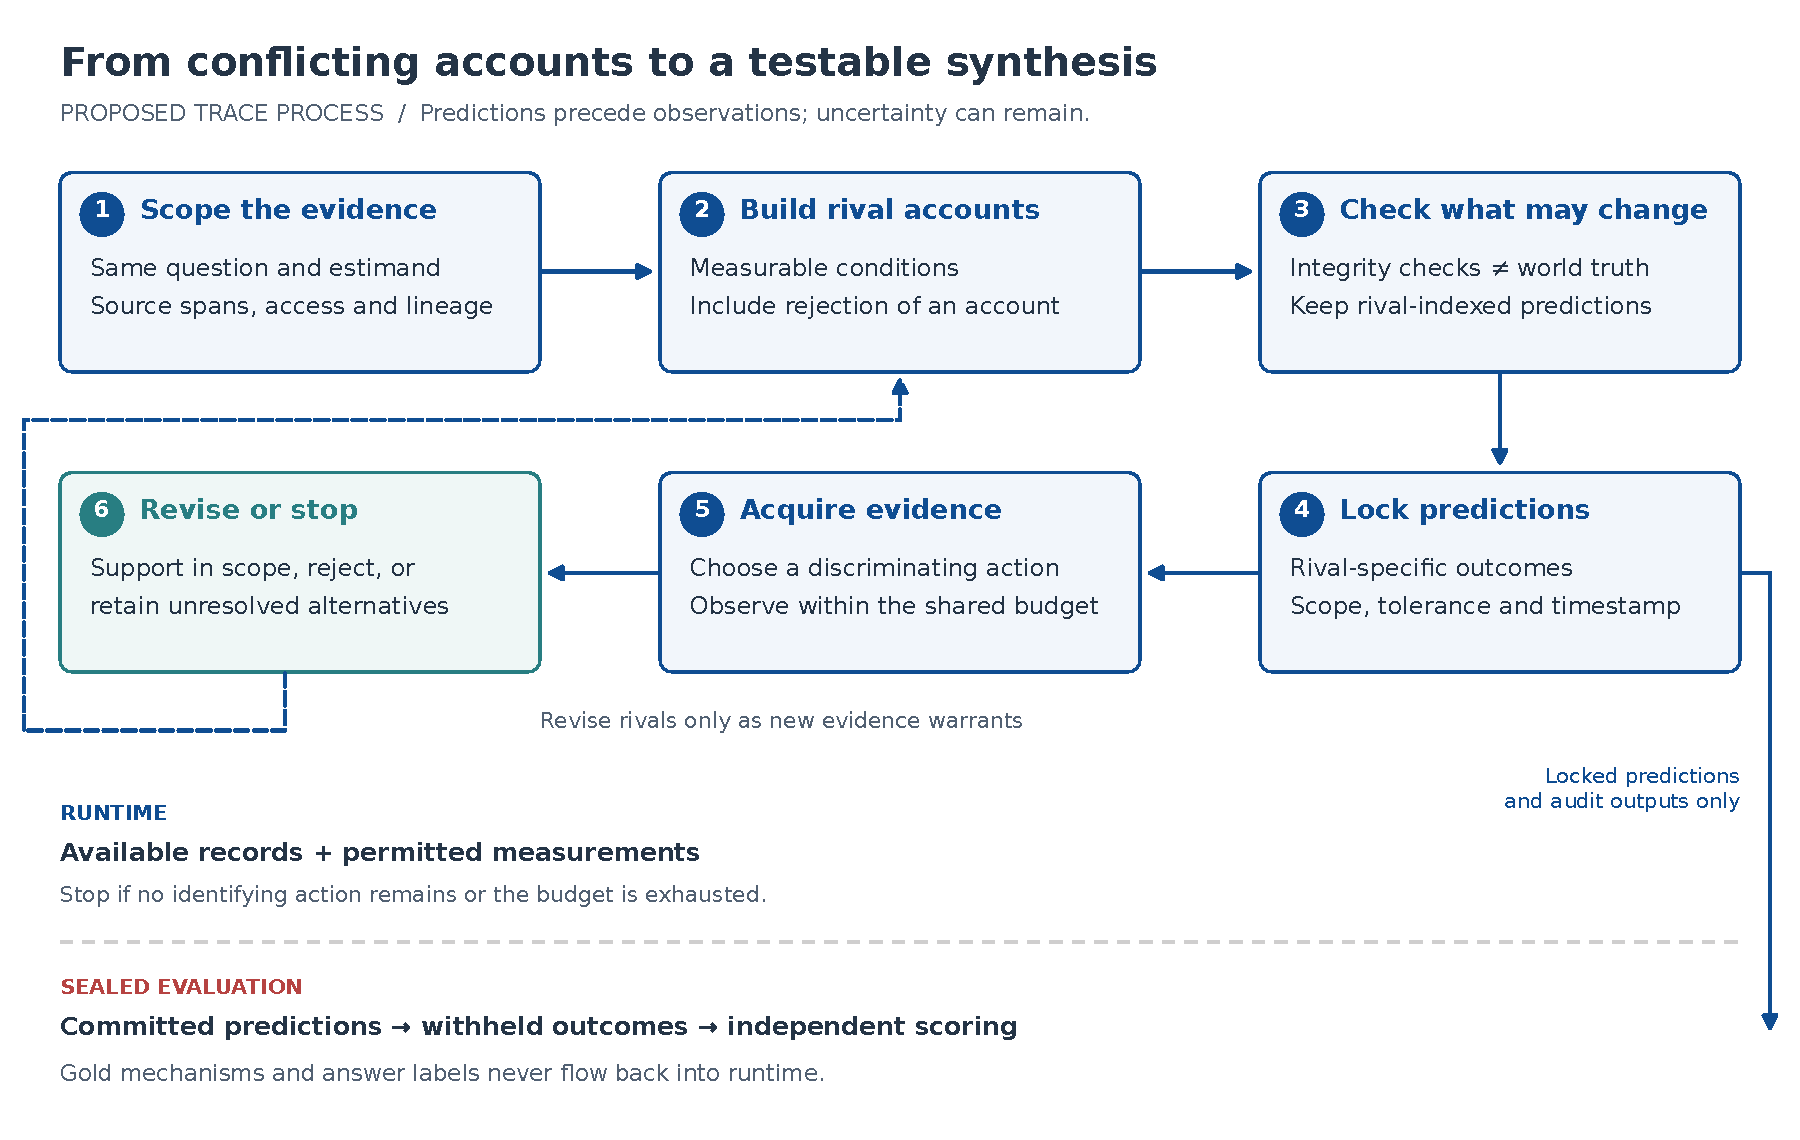
\includegraphics[width=\linewidth]{figures/trace-discovery-loop.pdf}
\caption{Proposed discovery loop. Integrity checks and rival-indexed predictions precede acquisition. Only committed outputs cross into sealed evaluation; no gold outcomes return to runtime.}
\label{fig:trace-discovery-loop}
\end{figure}

\par\medskip
\noindent\begin{minipage}{\linewidth}
\begin{CNSAlgorithm}
INPUT: source packet, questions, permitted actions, resource budgets
1  Extract source-linked claims, assumptions and observations.
2  Align questions; apply valid unit mappings; preserve unknowns.
3  Account for measurement lineage; record conflicts and context gaps.
4  Generate typed rivals and variable measurement requirements.
5  Validate dependencies; compile eligible numerical rules.
6  Rank proposals; activate at most four; preserve pending candidates.
7  Lock predictions before observation; run integrity checks.
8  Select a separating action or a logged prerequisite measurement.
9  Acquire within budget; update records and candidate adequacy.
10 Regenerate at most once; preserve all earlier commitments.
11 Assign warranted conclusions or unresolved status; export records.
OUTPUT: conflict, candidate, prediction, action and decision tables
\end{CNSAlgorithm}
\end{minipage}\par\medskip

A contract should not be validated by the same example whose result it
was invented to rationalize. Development can refine the grammar and
validator; calibration can tune abstention; confirmatory cases must be
new. The system may request a measurement from an outcome service, but
that service must return an ordinary reading rather than a hidden label
such as ``hypothesis true.'' The benchmark evaluator sees sealed
mechanisms and withheld predictions \textbf{only after} the runtime
outputs have been committed \citep{G08}.

Validation should be adversarial. A candidate that says ``the cache
helps exactly when it helps'' is circular. A rule invented solely to
rescue every negative example is disallowed by specified rule grammar
and held-out tests. A stable false answer fails external correctness. A
continually abstaining system fails coverage. A model that always
reconciles fails on direct-rejection controls. Conversely, a model that
refuses to synthesize whenever sources disagree should fail
discovery-eligible cases. These negative cases test whether the
procedure can reject inappropriate synthesis.

\section{Worked example: caching, mechanisms and
refutation}\label{worked-example-caching-mechanisms-and-refutation}

\begin{figure}[htbp]
\centering
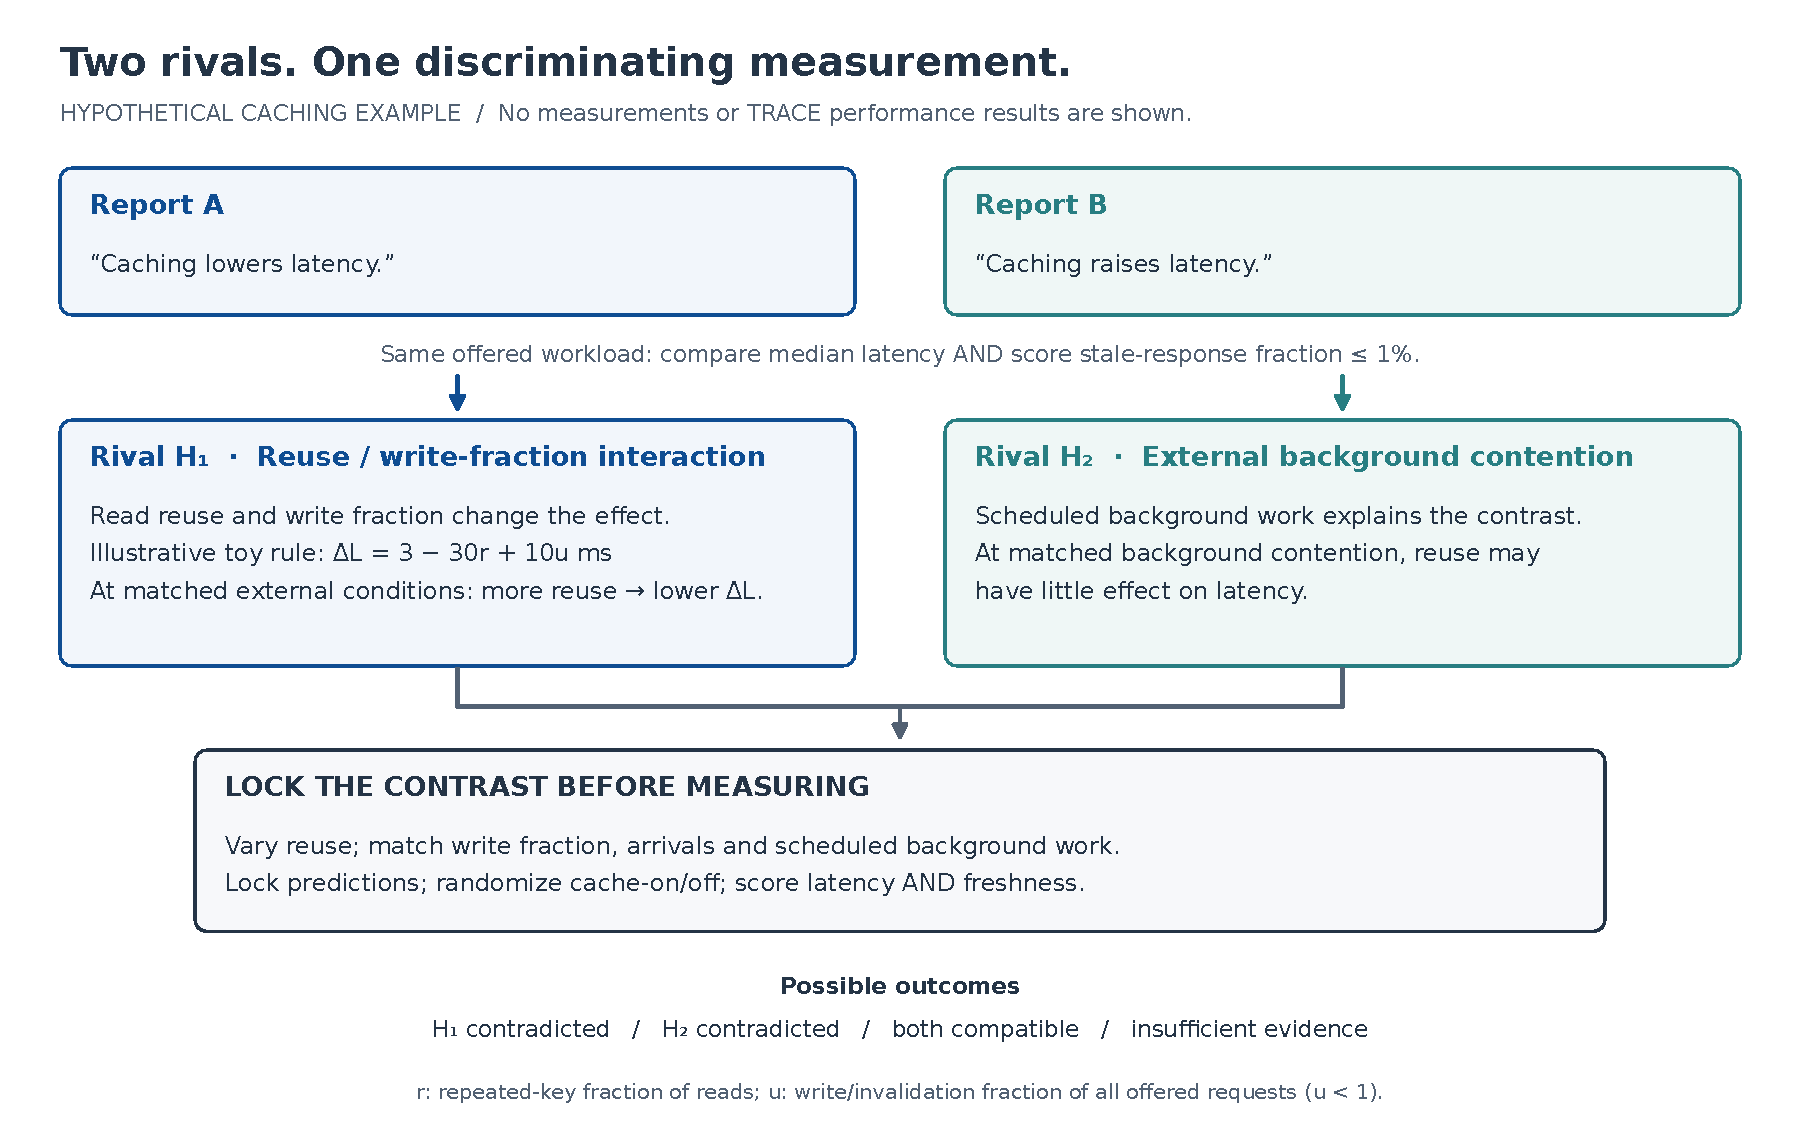
\includegraphics[width=\linewidth]{figures/trace-caching-example.pdf}
\caption{Hypothetical caching contrast. Reuse/write-fraction and external-contention rivals commit predictions before a separating measurement. Downstream utilization is not held fixed; latency and freshness are both scored.}
\label{fig:trace-caching-example}
\end{figure}

Figure 2 is a \emph{hypothetical illustration}, not a TRACE run. Define
\(\Delta L=L_{\mathrm{cache\ on}}-L_{\mathrm{cache\ off}}\) in
milliseconds for a fixed offered workload. Negative values indicate
lower median latency. Separately predict and measure staleness; a
workload is a deployment-success case only if its declared freshness
bound (for example, stale-response fraction at most 0.01) is satisfied.
Do not drop freshness failures after seeing them or condition the
latency estimate on selected successful requests.

Let \(r\) be the fraction of \textbf{read requests} repeating a key
already requested within a prespecified reuse window, and \(u\) the
fraction of \textbf{all offered requests} that are writes/invalidation
requests. Both are dimensionless workload settings, not an observed
cache-hit rate or writes per second. The denominator of \(r\) requires
\(u<1\); feasible key schedules, arrival rate and request mix must be
specified. A relation for communication only is

\[
\Delta L_{\mathrm{toy}}=(3-30r+10u)\ \mathrm{ms},\qquad 0\le r\le1,\quad0\le u<1.
\]

This invented relation illustrates a possible data-generating mechanism.
The TRACE numerical compiler fits piecewise-constant approximations to
observations; it does not infer the displayed formula or its
coefficients from prose. Two reports do not identify its coefficients.
Rival \(H_1\) proposes dependence on reuse and write fraction. Rival
\(H_2\) proposes that \textbf{externally scheduled background
contention} explains the contrast. External offered traffic and
background work can be controlled; backend utilization caused by cache
hits is a mediator, not a quantity to match across treatment arms.
Concurrency policy, hardware capacity, payload distribution and
reuse-window definition must also be fixed or explicitly varied.

Before observing a new workload, lock each rival's latency and freshness
predictions. A feasible contrast varies reuse while matching write
fraction, offered arrival rate and scheduled background contention; a
complementary contrast varies external contention at matched workload
settings. Randomize cache-on/off order and monitor carryover. Do not
artificially hold downstream CPU/database work constant while claiming
the total caching effect. If neither contrast separates the rivals,
record that limitation. If all candidates fail noise-aware adequacy
checks, reopen within budget or remain model-inadequate.

The cross-case record makes this example operational. Suppose background
work is recorded in report B but absent from A. The conflict row
identifies the incompatible latency generalizations and this context
gap. A candidate names contention as \CNSIdentifier{observed\_asymmetric},
retains the two reported measurements, and adds the hypothesis that
contention changes the caching effect. An action requests A's missing
context or a permitted matched workload. Its response populates an
observation row; it cannot retroactively alter the candidate's earlier
commitments. A mechanistic candidate may instead propose a new
measurable factor as \CNSIdentifier{inferred\_unmeasured}, with a measurement
procedure and a falsifiable prediction. If no action can measure it and
no justified prediction is available, it remains pending.

\textbf{What would distinguish TRACE here?} Every comparator receives
the same report spans, workload facts and available measurements.
Ordinary refinement and the Contrastive Discovery adaptation may
discover reuse, write fraction or contention without supplied
localization. TRACE additionally organizes the conflicting latency
generalizations and their missing-context links; its lineage variant
accounts explicitly for shared measurement origins. The example
establishes no advantage. Only a different, valid candidate pool
followed by stronger sealed predictions at matched cost would support
the localization hypothesis. Naming the same moderator more fluently
earns no credit.

Other outcomes follow the same record path. A milliseconds/seconds
difference yields a validated mapping and an alignment decision, with no
H2 discovery credit. A p99/median difference yields distinct questions.
Copied reports yield a lineage adjustment without a truth verdict. Rival
causal accounts that no permitted action separates yield unresolved
decisions. These records permit comparisons of failure and resolution
types across cases while preserving their evidential differences.

The prospective evaluator scores commitments against withheld
measurements collected later. Runtime may receive only the outcomes of
permitted acquisition actions, not gold mechanisms or evaluation
verdicts. The same extracted measurements must be available to direct
rule/regression learners. Correct predictive scope need not identify a
unique causal graph; causal wording requires defensible interventions
and assumptions.

\section{Primary question and supporting
hypotheses}\label{primary-question-and-supporting-hypotheses}

\textbf{H2 --- Independently predictive discovery (primary).} Does
explicit conflict localization improve the discovery of measurable
conditions beyond an established contrastive-discovery adaptation
receiving the same source facts? The primary comparison is C versus B in
Section 8. Each system locks its explanatory relationship, parameters
and final candidate before receiving the five prediction contexts. It
then applies that fixed candidate to those contexts and commits the
outputs before any outcome is revealed. All systems receive the same
context fields from a task dictionary fixed during development; field
selection must not disclose the correct moderator. New variables require
an operational mapping to available fields or remain unmeasured. The
evaluator selects challenge settings before generation, independently of
each system's proposals. Success requires a source-faithful explanatory
relationship not explicitly supplied in the packet, a distinguishing new
prediction, and at least four of five predictions correct under frozen
tolerances, including every prespecified diagnostic setting needed to
distinguish the task's principal unconditional alternative. Alignment,
copying detection and restatement earn no discovery credit. Candidate
novelty is relative to the initial packet, not a claim of novelty to
science. A condition may be new even when its variables occur in the
reports; what must be absent is the explanatory relationship. No credit
requires guessing an unobservable latent variable. A blinded semantic
rubric and held-out prediction scoring assess different requirements;
neither substitutes for the other.

The generation-only study uses a fixed permitted evidence snapshot. A
variable absent from the measurements can support a conjecture, but
unsupported assignments cannot manufacture fit or warrant. A case
needing further measurements remains pending on the static branch;
discovery following acquisition belongs to the subsequent adaptive
study. Each positive challenge set must distinguish a plausible
unconditional alternative; use mixed regimes and boundary settings where
appropriate, rather than require sign reversals for every mechanism
family.

\textbf{H1 --- Reliability (supporting quality measure).} Report
base-answer correctness, response to nuisance and relevant changes,
coverage, false promotion and unsupported resolution. A system that wins
H2 by inventing conditions indiscriminately or refusing difficult cases
has not established a useful discovery method. Include negative controls
where no new condition is justified and cases where accessible evidence
cannot identify the answer. Report denominators and unconditional
scores; do not select only successful generations for analysis.

\textbf{H3 --- Investigation (conditional subsequent study).} Only after
the representation and generation stages show credible predictive value,
compare evidence acquisition against Contrastive Discovery, POPPER where
its statistical assumptions can be met, ordinary experimental design and
simple random/relevance policies. All receive the same action access and
costs. The endpoint is an evidence-supported scoped conclusion within
budget, not the number of self-declared resolved questions. Static and
adaptive outcomes remain separate.

H2 is the scientific priority. H1-only improvement supports a narrower
reliability tool; H3-only improvement may support ordinary active
learning. Neither rescues a failed claim about conflict-conditioned
discovery. No superiority, fixed effect size or statistical power is
claimed for the exploratory pilot.

\section{Proposed evaluation design and decision
gates}\label{proposed-evaluation-design-and-decision-gates}

\subsection{Development and exploratory
pilot}\label{development-and-exploratory-pilot}

Start with \textbf{12--20 manually inspected development cases}. Include
genuine same-estimand conflicts, apparent unit/measurement differences,
copied sources, asymmetric missing context, an unstated measurable
condition and non-identifiable alternatives. Use the eight mechanism
families as a coverage taxonomy, not a forced equal-size factorial grid.
Experts must check whether the target is identifiable from each
permitted evidence view and whether the five withheld settings can
distinguish a plausible wrong rule. A realistic source packet may
contain several issues at once.

Then freeze the extractor, models, prompts, schemas, candidate limits,
tolerances, costs, adjudication rubric and scoring process for a
separate \textbf{30--60-case exploratory pilot} with unseen outcomes and
disjoint generating episodes/source clusters. These counts diagnose
feasibility; they are not powered sample sizes for a superiority claim.
Include eligible discovery cases and prespecified
no-discovery/non-identifiable controls; publish their actual counts and
uncertainty separately. Eligibility is fixed before any system runs; all
eligible cases remain in the H2 denominator, including abstentions,
invalid outputs and missing predictions. Control strata have their own
denominators. Case selection must not depend on TRACE succeeding or
competitors failing. Family labels and eligibility certificates remain
evaluator-only.

All development and pilot cases produce the common records in Section
4.1. Repeated prompts, five predictions, source copies and model seeds
are not independent research cases. Pilot revisions require fresh cases
for a subsequent evaluation. No benchmark data, pilot or implementation
has yet been produced.

\subsection{Identical facts, different evidence
organization}\label{identical-facts-different-evidence-organization}

The common-input study freezes source-linked questions, measurements,
missingness, report text and available lineage facts. An evaluator may
certify targets but must never supply the true moderator or causal
mechanism to runtime. All systems can inspect the same original spans
and infer their own conflicts or dependencies.

\begin{longtable}[]{@{}
  >{\raggedright\arraybackslash}p{(\linewidth - 2\tabcolsep) * \real{0.5000}}
  >{\raggedright\arraybackslash}p{(\linewidth - 2\tabcolsep) * \real{0.5000}}@{}}
\toprule\noalign{}
\begin{minipage}[b]{\linewidth}\raggedright
System
\end{minipage} & \begin{minipage}[b]{\linewidth}\raggedright
Proposed operation on the common evidence
\end{minipage} \\
\midrule\noalign{}
\endhead
\bottomrule\noalign{}
\endlastfoot
A & Strong iterative hypothesis refinement, with an additional
counterexample-prompting variant; adapted from established
hypothesis-refinement methods \\
B & Contrastive Discovery adaptation: explicit alternative explanations;
generation and scoring documented against the original method \\
C & Same scaffold as B, augmented with a generated conflict-alignment
record and conflict-directed generation; common row-based fitting and
warrant rules \\
D & Same as C plus explicit dependence-aware weighting and warrant
accounting from the available lineage facts \\
\end{longtable}

\textbf{C versus B is the primary comparison.} Both propose explicit
rival explanations. C receives an additional generated conflict record
and conflict-directed instruction; B may identify conflicts itself. Hold
the model, source packet, proposal capacity, prediction interface and
final selector fixed. This measures the localization package, not the
isolated effect of a single field or instruction. A matched auxiliary
condition gives B an equally budgeted source-summary call, using the
same evidence without instructions to localize conflicts. It tests
whether extra preprocessing explains an apparent gain. All preprocessing
consumes the common resource ceiling.

\textbf{Common selection.} After structural validation, a shared
selector receives source evidence and candidate predictions/assumptions,
with system identity, conflict IDs and generation order hidden. Order
candidates by coverage of observed contexts without invented values,
then fewer unsupported assumptions, then canonical candidate ID. Within
the numerical form, apply the same training-loss criterion and row
weights. This selector uses no test outcomes or localization-specific
score. It can select an unresolved result. Log candidate-pool quality
separately from the selected-candidate endpoint. The full TRACE ranking
in Section 4.3 is tested separately.

\textbf{Comparator fidelity.} B is a static adaptation of contrast-set
generation to a fixed evidence snapshot. It does not reproduce
Contrastive Discovery's adaptive search, and the common selector
replaces its native scoring for this mechanism experiment. Its
alternative set should cover a declared question with disjoint
explanations; log incomplete or overlapping coverage. An explicit
residual explanation means none of the specified explanations applies;
uncertainty about which explanation holds is a separate decision state.
Neither makes an arbitrary set logically exhaustive.

\textbf{Transfer to an existing discovery method.} Compare the same
capable discovery implementation with and without generated TRACE
conflict records. Preserve its native hypothesis generation, belief
scoring, search, revision and stopping rules; the intervention supplies
source-linked localization and instructions for using it, not TRACE's
selector or rule compiler. Both conditions receive identical source
facts and access to the same analysis service. Include an equally
budgeted source-summary condition. Charge extraction, localization,
elicitation, failed attempts and analysis to a common resource ceiling
established during development that permits the native workflow to
operate. Record any interface changes and pin code, prompts and model
versions. Sealed outcomes remain inaccessible to all search tools. At
the budget boundary, lock each method's selected explanation and use the
same outcome-blind prediction interface and held-out scoring; report
this external endpoint separately from native belief-based resolution.

Contrastive Discovery is the closest contrastive comparator, but its
author page lists code as forthcoming. A paper-based implementation must
be labeled a reproduction attempt, with unresolved fidelity differences
disclosed. AutoDiscovery offers a released implementation for a
complementary transfer comparison; its current defaults differ from its
paper and must not be presented as the original experimental
configuration. Report either comparison separately from static C--B, and
report adaptive evidence acquisition separately from fixed-evidence
analysis. Belief scores are not correctness labels. If the native
procedure cannot operate within the task interface, disclose the
incompatibility. A static C--B gain supports that scaffold-specific
intervention; evidence for a transferable component requires improvement
within an existing method with its native scoring and search preserved.

\textbf{D versus C tests lineage handling}, not the benefit of giving D
extra source facts. Both receive identical lineage metadata; C can
reason about it ordinarily, while D applies explicit accounting. In the
controlled compiler, B/C use row-based fitting and D uses the
lineage-aware fitting and eligibility rules in Section 4.4. The
comparison therefore isolates the accounting package, not an information
advantage. A full two-by-two localization/lineage factorial can be added
if interaction is itself a research target. Without that factorial, D--C
is conditional on localization and cannot establish an independent main
effect of lineage.

The common-input experiment tests evidence organization on a frozen,
source-faithful extraction. Because that extraction may favor some
methods, its errors and construction procedure must be disclosed. Also
run an equal-access end-to-end comparison in which extraction and
localization are generated separately for each method and all their
costs/errors count. Common-input records produced by TRACE must not
contain its inferred answer. Human-corrected conflict records are an
oracle diagnostic reported separately, never the primary result. Freeze
provenance of every field so an apparent algorithmic advantage cannot
conceal additional information.

Retain an ordinary common-extractor rule/tree/regression learner (B8),
with exhaustive search when inexpensive. It tests whether tabular
learning explains any gain. A and B should receive serious development
tuning, the same evidence and comparable tuning resources; the
counterexample-prompting control tests whether a simple instruction
captures the effect. Prior RAG, verification, debate, AAL-sketch and
CNS-subset comparators are optional diagnostics rather than a mandatory
ten-system first study. Our AAL implementations remain
operationalizations of Lopez-Paz's sketch, not author-released systems.

\subsection{Outcomes, budgets and causal
attribution}\label{outcomes-budgets-and-causal-attribution}

Score the final locked candidate per case, all five predictions, and all
invalid or missing outputs. Report the H2 success proportion, prediction
loss, source-fidelity errors, new measurable candidate yield,
false-condition promotion, unsupported resolution, coverage and actual
cost. Log every proposed candidate before selection so a predictive gain
can be distinguished from more proposals or better selection. Candidate
equivalence is judged through variable definitions, relationships and
predicted consequences rather than different prose alone; adjudicators
are blinded to system identity and disagreements are retained. For
continuous targets, the primary correctness score uses a point
prediction and a tolerance fixed from the measurement design; each
candidate cannot choose its own acceptance width. For categorical
targets, require one category. Optional uncertainty intervals are scored
separately with a width-sensitive rule, and probabilistic forecasts with
an appropriate proper score. Wide intervals and multiple guesses cannot
satisfy the primary prediction gate. Specify how noisy repeated
measurements form the target estimate before unblinding.

Two independently blinded reviewers apply the source-fidelity and
packet-relative novelty rubric to candidate records. Resolve
disagreements with a third reviewer and report initial agreement and
unresolved cases. Human decisions never return to runtime. On the small
pilot, inspect all cases rather than extrapolate from a favorable
subset. Outcome scoring uses the frozen executable rule wherever
possible.

For TRACE and the controlled B/C scaffold, start with one shared
extraction, one preprocessing call per condition, up to eight proposals,
one structural repair and at most four active rivals. The common
selector is also charged. Faithful iterative or adaptive method-level
competitors may divide the same total budget differently. For the pilot,
propose a common per-case ceiling of 16,000 input and 4,000 output
tokens across all static stages, including extraction, localization and
repair. Context packing must preserve the same evidence across systems;
if this is infeasible, change the setting during development, then
freeze it. Report usage rather than require waste to equalize totals.
Measure CPU time for ordinary learners and model tokens, calls and
latency for every method. Generated localization consumes the common
budget; an oracle-localization result is a separate diagnostic.

Freeze one model/version and seed for the exploratory primary
configuration; additional seeds are paired sensitivity runs. In
candidate-generation comparisons, common compilation and scoring follow
generation. In prioritization diagnostics, freeze the candidate pool and
vary only ranking. In numerical search-order diagnostics, freeze the
extracted table and rule language, compare contrast order, seeded
permutation and exhaustive enumeration, and report the complete cost
curve. These are different interventions.

\subsection{Interpretation and stop
decisions}\label{interpretation-and-stop-decisions}

Report paired case-level differences and uncertainty, errors by case
type, all exclusions and the full candidate/commitment records. The
pilot is exploratory: neither a favorable p-value nor four correct
predictions in one case demonstrates scientific superiority. State the
sampled population and source clustering before selecting an interval
method; avoid a nominal precision calculation that treats related
packets as independent. Do not infer equivalence from a nonsignificant
difference.

Proceed through four gates: \textbf{representation}, can claims, scope
and lineage be extracted without unsupported values;
\textbf{generation}, does localization produce different measurable
candidates from B; \textbf{prediction}, do those candidates improve
sealed predictions without unacceptable false promotion or coverage
loss; \textbf{cost and transfer}, does the pattern survive metered
budgets and genuinely different case construction? Publish paired
estimates at every gate. Gates guide continuation, not post hoc
filtering of reported failures. If candidate content and frequency are
similar but selection improves, investigate selection as the mechanism.
If neither candidate yield nor sealed prediction shows useful change,
stop scaling until a concrete repair warrants fresh cases. A small
inconclusive pilot warrants an uncertainty assessment, not a declaration
that the methods are equivalent.

Before a confirmatory study, choose a smallest worthwhile effect and
safety margins with domain justification; estimate paired discordance
and source clustering from development/pilot data; then select a sample
size with power and sensitivity calculations. Freeze the primary C--B
comparison, its independent unit, valid interval/test, treatment of
invalid outputs and multiplicity family. D--C and other comparisons
remain secondary unless additional error control is specified. The pilot
cannot certify a 5\% false-promotion ceiling on a small control stratum.
Report exact counts and sampling-appropriate uncertainty instead of
treating absence of observed errors as safety.

Stop or reduce the proposal if ordinary refinement or contrastive
discovery produces equivalent candidates and predictions at lower cost,
if localization mainly inserts unsupported assumptions, or if all
benefit is extraction/deduplication. A useful benchmark or reliability
tool would require its own contribution argument; neither is an
automatic consolation prize. If prior work already specifies the same
operational distinction, withdraw the methodological claim rather than
add machinery to protect it.

\subsection{Conditional extensions}\label{conditional-extensions}

A later H3 study may use the same three-action/12-cost-unit engineering
ceiling, but must define action costs and identifying evidence
independently of the hidden answer. A faithful POPPER comparison
requires valid test statistics and implication checks; when these are
unavailable, disclose incompatibility and report only a labeled
falsification-style adaptation without inheriting its statistical
guarantee. Compare full search policies separately from experiments that
hold the candidate pool fixed. TRACE's set-separation score is a
heuristic, not sequential error control.

Larger synthetic studies across F1--F8, source-clustered verification
panels, DiscoveryBench and prospective caching measurements remain
possible extensions \citep{R25, R26, R27, R28}. ConfRAG is an additional
conflict-reasoning diagnostic, not a substitute for predictive discovery
\citep{R44}. Sample sizes and execution counts for these extensions
require a separate design after feasibility is established. A
prospective study must first specify service regimes,
hardware/day/carryover blocks, withheld measurement collection after
commitment and uncertainty at the independent regime level. Workload
seeds and repeated requests do not establish independent mechanisms.

All phases require sealed evaluator outcomes, source-cluster separation,
immutable prediction commitments and publication of failures. Runtime
receives only permitted records and measurement results, never gold
mechanisms, eligibility labels or evaluator judgments. Leakage, changed
tolerances after unblinding or source overlap invalidate confirmatory
interpretation.

\section{Relationship to earlier CNS and design
choices}\label{relationship-to-earlier-cns-and-design-choices}

\begin{figure}[htbp]
\centering
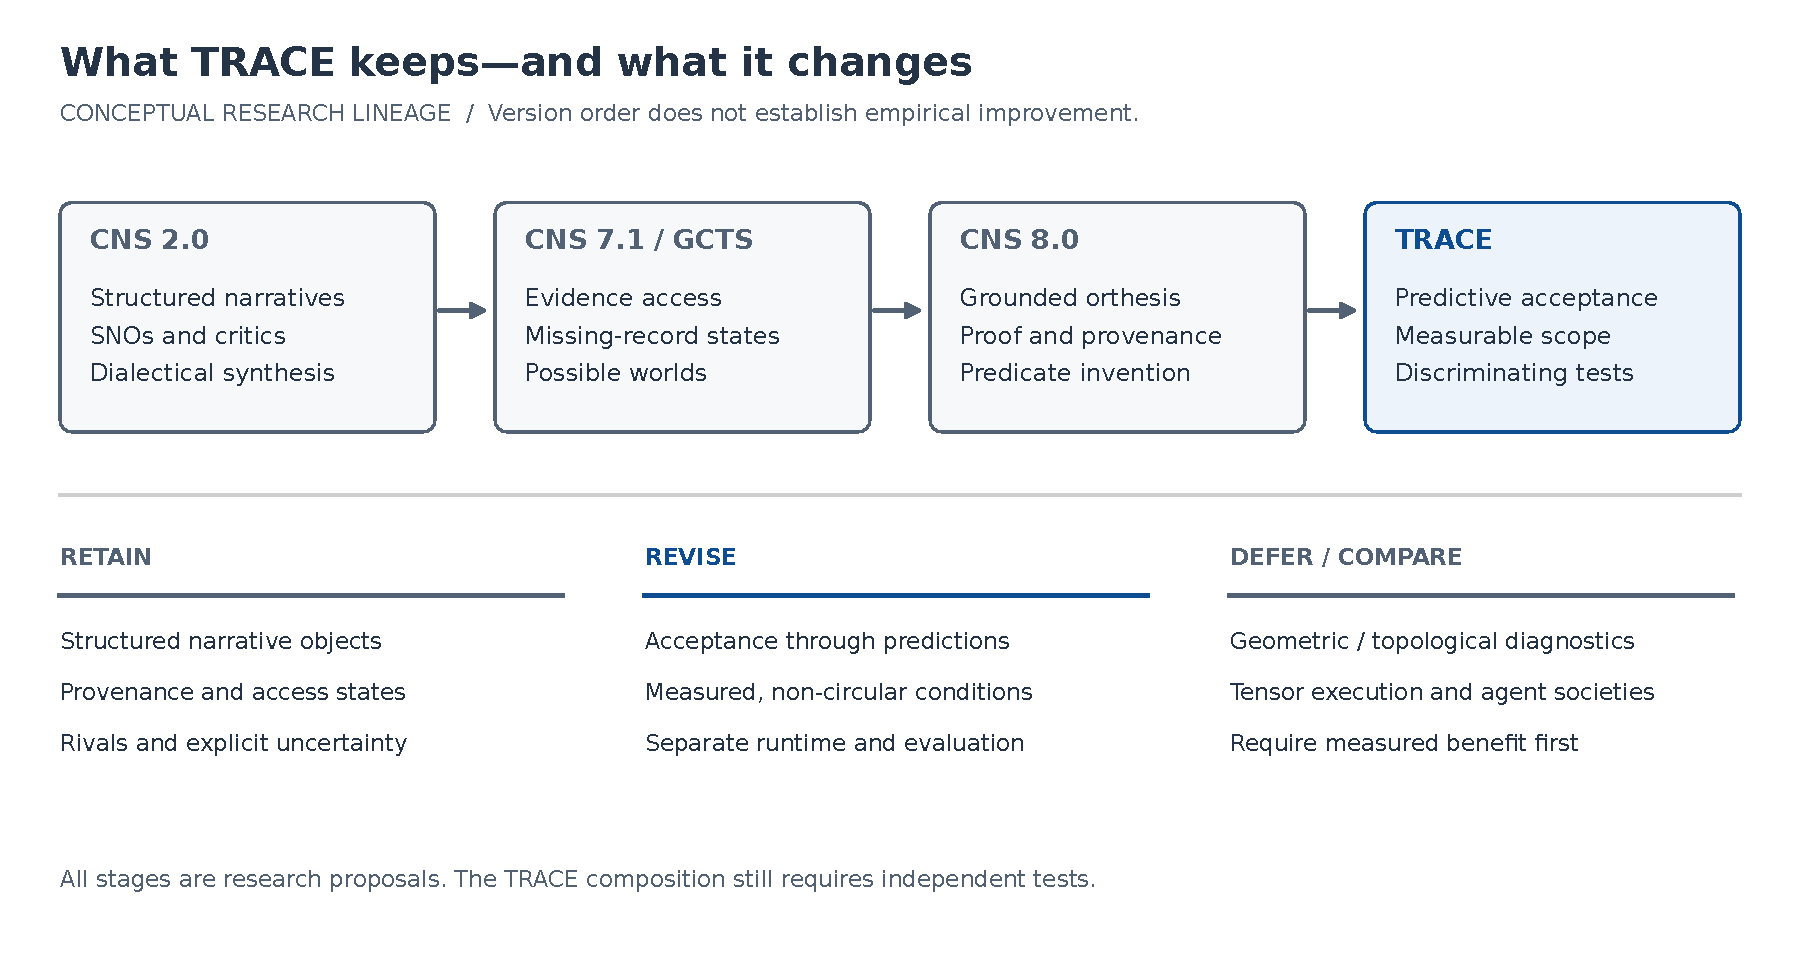
\includegraphics[width=\linewidth]{figures/trace-research-lineage.pdf}
\caption{Conceptual research lineage, not measured improvement. TRACE retains structured evidence and uncertainty while evaluating predictive acceptance against simpler alternatives.}
\label{fig:trace-research-lineage}
\end{figure}

Figure 3 depicts conceptual lineage rather than measured improvement.
CNS 2.0 introduced a research program around SNOs, chiral opposition and
criticism; GCTS 7.1 emphasized grounded evidence and access-state
distinctions; CNS 8.0 restored synthesized SNOs and proposed orthesis
conditions, proof traces and predicate invention with complexity limits
\citep{G13, G11, G02, G09}. CNS 8.0 already states that orthesis
stability is not metaphysical truth and can preserve unresolved
contradictions. TRACE develops this lineage through predictive
acceptance criteria and explicit comparison of explanatory accounts.

The proposal retains structured accounts, provenance, versioned
revisions, rival interpretations, and the ability to construct a
conditional new account. It revises the meaning of productive conflict:
shared target, explicit evidentiary relationships and \textbf{testable
differences in predictions} matter more than a single combined chirality
score. The previous literature's use of ``Evidential~Entanglement''
conflated at times shared evidence identifiers with comparable study
endpoints; TRACE records semantic comparability, shared records and
source copying independently \citep{G09}.

Proof closure remains useful for checking derivability from stipulated
premises. Round-trip language-to-logic fidelity remains useful for
identifying translation errors. Both checks concern the representation
and its premises; neither independently verifies the world claim.
Manifold geometry, curvature, holonomy, topological reduction, tensor
execution and large multiagent societies are \textbf{optional future
comparators}, not prerequisites. They should return only if a specific
reproducible task demonstrates gains beyond simpler representations at
acceptable cost. The original work is preserved as prior art rather than
rewritten as validated implementation evidence.

\section{Risks, limits, and alternative
explanations}\label{risks-limits-and-alternative-explanations}

\textbf{Admissibility is underspecified in the world.} A model may call
a transformation irrelevant even though it changes the question, or
reject a relevant change because it undermines a preferred answer.
Independently reviewed development contracts and held-out contract
families reduce---but cannot eliminate---this risk. Unresolved contracts
retain their unknown status in the output.

\textbf{The hypothesis interface introduces bias.} The numerical
compiler can miss relationships outside its rule language. Generated
mechanisms can also omit relevant variables or rely on unsupported
assumptions; an executable prediction does not remove that risk.
Expanding the language risks overfitting, combinatorial search and post
hoc excuses. The primary study should report both failures to represent
the truth and unjustified inventions; neither can be cured silently
after unblinding.

\textbf{Synthetic worlds may reward the generator's assumptions.} A test
set built from the designer's mechanism families can privilege
algorithms that match those families. External tasks, unseen families
and prospectively acquired data must therefore count heavily in
interpretation, even though none establishes universality. Publication
of generator code after evaluation is necessary but not sufficient if
the models' training corpora contain familiar templates.

\textbf{Evidence is not independent just because prose differs.} Copied
records, model-generated perspectives and repeated calls may share the
same error. The dependency graph itself can be uncertain. A fair
comparison must give baseline systems the same provenance fields and
assess the ability to detect unknown dependencies rather than scoring a
fabricated certainty.

\textbf{Observation policy can be harmful or uninformative.} High
information gain may target the wrong hypothesis class or exceed a
privacy, safety, or resource budget. The first prospective example is a
sandboxed software service, not human subjects or clinical
interventions. External actions require domain-specific permission and
governance; the proposal confers no authority to run arbitrary
experiments.

\textbf{The explanatory narrative may be unfaithful.} A plausible causal
sentence is not proof of the model's actual inference process
\citep{R18}. The deliverable should be a compact, source-linked and
checkable claim, its prediction record and its test outcome. Causal
language should be reserved for designs where the identification
assumptions are defensible.

\textbf{Alternatives may explain any future gain.} A structured SNO
schema, more compute, a better retrieval index, source deduplication,
direct regression, or simpler active learning could capture all apparent
improvement. The proposed ablations and well-resourced baseline suite
are required to distinguish the proposed mechanism from these
alternatives.

\textbf{The ambition is domain-limited.} Scientific and software
observations sometimes admit controlled interventions and clear metrics.
Historical claims, sparse observational science and normative
disagreement may not. TRACE must say ``unresolved'' where there is no
permitted identifying observation, rather than imply that every
contradiction hides a discoverable conditional truth.

\section{Research agenda and
conclusion}\label{research-agenda-and-conclusion}

The immediate work is a faithful representation and comparator exercise
on a small development set, followed by a frozen exploratory pilot.
Sections 4.1--4.6 define interfaces for that exercise; they do not
require a production agent platform before the central comparison can be
examined. Expert review should challenge source fidelity, comparator
adaptations and case identifiability before more resources are
committed.

TRACE asks whether localized disagreement between documented accounts
adds predictive value beyond existing contrastive and abductive
discovery methods. The common records and controlled comparisons specify
what evidence would answer that question. A contribution requires
demonstrated incremental value and adequate differentiation from prior
work. If the primary comparison fails, the appropriate outcome may be a
simpler reliability tool, a separately justified benchmark, or
retirement of the proposed method.

\section{Citation and version note}\label{citation-and-version-note}

\textbf{GTCode.com (15 November 2026).} \emph{TRACE: Contrast-Guided
Discovery from Conflicting Accounts}. Research proposal, version 0.1.
Canonical edition: \textbf{https://gtcode.com/papers/trace/}. This
version is not peer reviewed, not preregistered, and contains \textbf{no
TRACE experimental results}. The web research article, the compiled PDF,
and the supplied LaTeX source correspond to the same v0.1 substantive
manuscript. A public companion
\href{https://gtcode.com/guides/trace/overview/}{overview} and
\href{https://gtcode.com/guides/trace/evaluation/}{proposed evaluation
specification} are separate interpretive and protocol documents.

\bibliographystyle{unsrtnat}
\bibliography{references}
\end{document}
